\documentclass[a4paper,11pt]{article}
\usepackage{fullpage}
\usepackage[latin1]{inputenc}
\usepackage[T1]{fontenc}
\usepackage[normalem]{ulem}
\usepackage[english]{babel}
\usepackage{listings,babel}
\usepackage{palatino}
\usepackage{gensymb}
\lstset{breaklines=true,basicstyle=\ttfamily}
\usepackage{graphicx}
\usepackage{moreverb}
\usepackage{url}
\usepackage{tabularx}
\usepackage{float}
\usepackage{tweaklist}
\renewcommand{\itemhook}{\setlength{\topsep}{0pt}\setlength{\itemsep}{0pt}}
\renewcommand{\enumhook}{\setlength{\topsep}{0pt}\setlength{\itemsep}{0pt}}

\title{TDC Core Test Report}
\author{S\'ebastien Bourdeauducq}
\date{November 2011}
\begin{document}
\setlength{\parindent}{0pt}
\setlength{\parskip}{5pt}
\maketitle{}
\section{The demonstration design}
\subsection{Hardware}
The demonstration design runs on a SPEC board equipped with a FMC DIO 5-channel daughterboard.

Data is transferred at 115200 8-N-1 via the serial console accessible using the built-in USB adapter. The PCIe interface is not used.

Test signals go through the FMC daughterboard. The first LEMO connector on the daughterboard is configured as output and transmits an oscillating pattern. The next two LEMO connectors are inputs connected to TDC channels.

For measuring the FPGA temperature, the 1-wire sensor IC19 is placed on top of the FPGA using kapton tape. Thermal paste improves conduction between the FPGA and the sensor.

\subsection{Contents}
The demonstration design contains:
\begin{itemize}
\item the LatticeMico32 soft processor, running at 125MHz from the clock generated by the CDCM61004 chip on the SPEC.
\item UART, timer and GPIO cores from the Milkymist SoC. Memory-mapped.
\item the TDC core with its Wishbone interface, configured for two channels, also clocked from the 125MHz source. Memory-mapped.
\item a ring oscillator for startup calibration of the TDC core.
\item an oscillator for generating TDC test signals.
\item a basic boot ROM and command line interface based on the Milkymist BIOS.
\item software routines for testing the TDC core.
\end{itemize}

\subsection{TDC core implementation details}
The TDC core is implemented with the following parameters:

\begin{center}
\begin{tabular}{|l|c|}
\hline
g\_CHANNEL\_COUNT & 2 \\
\hline
g\_CARRY4\_COUNT & 124 \\
\hline
g\_RAW\_COUNT & 9 \\
\hline
g\_FP\_COUNT & 13 \\
\hline
g\_EXHIS\_COUNT & 5 \\
\hline
g\_COARSE\_COUNT & 25 \\
\hline
g\_RO\_LENGTH & 31 \\
\hline
g\_FCOUNTER\_WIDTH & 13 \\
\hline
g\_FTIMER\_WIDTH & 14 \\
\hline
\end{tabular}
\end{center}

To minimize variations of the timing properties between runs of the automated place and route tool and to maximize thermal coupling between each delay line and its online calibration oscillator, the design is floorplanned.

The two delay lines from each channel are placed close to their respective IOBs. Because of their large height, there are few FPGA columns that can accomodate them, and they accidentally ended up close to each other. The ring oscillator components are placed in the SLICEX columns just at the right of the delay lines, and spread evenly along the height of the delay lines. This is illustrated by Figure \ref{fig:floorplan}, where the delay lines are colored pink and the ring oscillators are yellow.

In the UCF file, this is achieved by manually placing the first CARRY4 primitive in each delay line. Since carry chains can only be placed in columns, this determines the placement for the complete delay line. For the ring oscillators, a Python script generates one placement constraint for each element.

\begin{figure}[H]
\centering
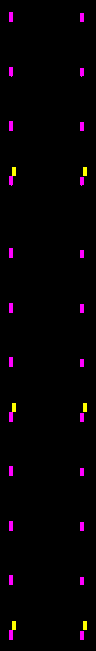
\includegraphics[width=1.6cm]{floorplan.png}
\caption{Floorplan of the delay lines and ring oscillators in FPGA Editor.}
\label{fig:floorplan}
\end{figure}

In the input signal path, there are one multiplexer and one inverter per channel. Everything is packed into one FPGA slice, which is also manually placed to minimize timing variations. The physical input signal path can be seen in Figure \ref{fig:inputpath}. The LVDS IOBs are represented in blue, and the routing and the slice in green.

A limitation of this TDC design is that it does not compensate for PVT variations in the input signal path elements.

\begin{figure}[H]
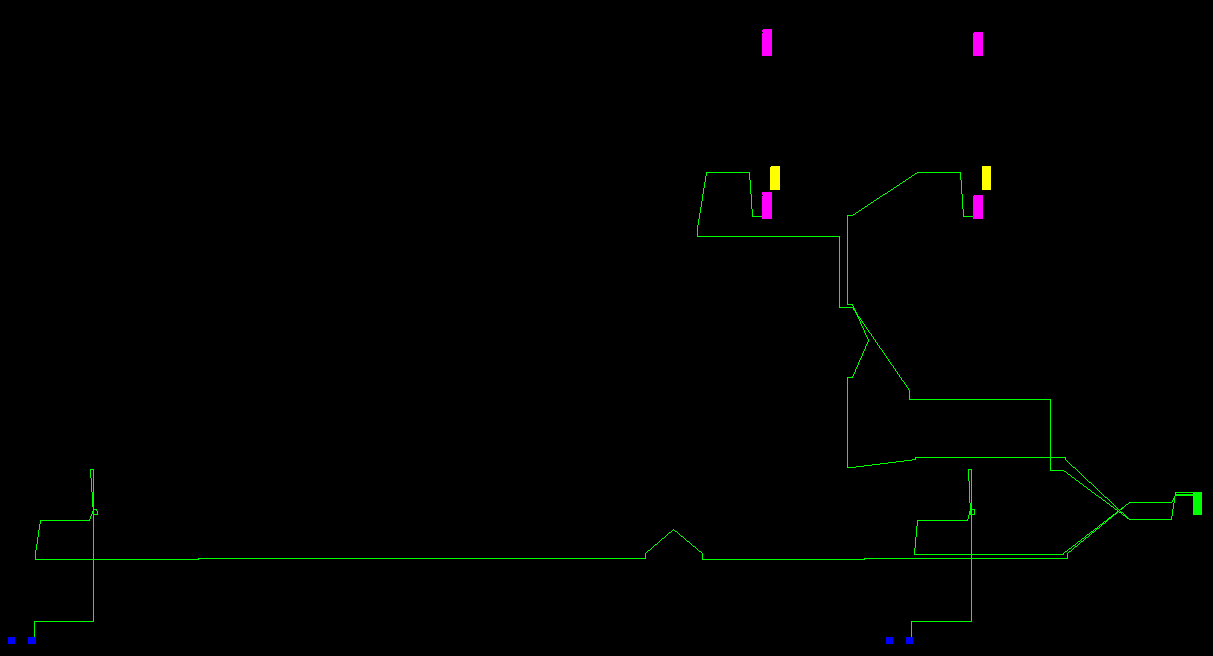
\includegraphics[width=\textwidth]{input_routes.png}
\caption{Input signal path in FPGA Editor.}
\label{fig:inputpath}
\end{figure}

\subsection{Synthesizing and running the design}
\subsubsection{Compiling the LM32 software}
Since the LM32 software is used in block RAM initialization, it must be compiled before the FPGA bitstream is built. The scripts expect the lm32-rtems4.11 GCC toolchain, but any LM32 toolchain should be suitable.

You will need first to compile some host tools which are used to build block RAM initialization files:
\begin{verbatim}
cd $TDCDIR/demo/tools
make
\end{verbatim}

Then, compile the base library and the software image:
\begin{verbatim}
cd $TDCDIR/demo/software/libbase
make
cd $TDCDIR/demo/software/demo
make
\end{verbatim}

\subsubsection{Compiling the FPGA bitstream}
The design can be synthesized with ISE 13.2. You will also need Python to generate the floorplanning constraints. The compilation is automatic:
\begin{verbatim}
cd $TDCDIR/demo/boards/spec/synthesis
make -f Makefile.xst
\end{verbatim}

\subsubsection{Downloading the FPGA bitstream}
If you are using Xilinx iMPACT, there is an automatic script:
\begin{verbatim}
cd $TDCDIR/demo/boards/spec/synthesis
make -f Makefile.xst load
\end{verbatim}

Otherwise, load the file \verb!$TDCDIR/demo/boards/spec/synthesis/build/system.bit! with your favorite FPGA programming tool.

\subsection{Command line interface}
Once the bitstream is loaded, it implements a command-line interface on the serial console (115200 8-N-1), and it displays a \textbf{TDC>} prompt. From there, you can enter the following commands:

\begin{tabularx}{\textwidth}{|l|X|}
\hline
mr <address> [length] & Reads memory. Length is in bytes (default 1). \\
\hline
mw <address> <value> [count] & Writes one or several 32-bit words to memory. Count is in words (default 1). \\
\hline
temp & Displays the current temperature in \degree C measured by the 1-wire sensor. \\
\hline
rofreq & Outputs a series of comma-separated values representing the current temperature (in \degree C) and the ring oscillator frequencies (measured in counts) from each TDC channel. Sending any character to the console stops the series of measurements. \\
\hline
calinfo & Dumps the current contents of the histogram and the LUT for each TDC channel. \\
\hline
daclevel <value> & Sets the output voltage on all channels of the I2C DAC5578 digital to analog converter on the FMC DIO board. The 16-bit value is directly written into the DAC. \\
\hline
mraw & Outputs a series of raw (pre-LUT) measurements from the first TDC channel. Sending any character to the console stops the series of measurements. \\
\hline
diff & In a loop, waits for a TDC event to happen in both channels, and displays its parameters. The output is in CSV format and contains the following information: polarity for the first channel, raw timestamp for the first channel, fixed-point timestamp for the first channel, and the same for the second channel. Sending any character to the console stops the series of measurements. \\
\hline
\end{tabularx}

\section{Methods and results}

\subsection{Effect of temperature on ring oscillators}
\label{sec:rofreq}

The purpose of this experiment is to examine how temperature affects propagation delays. We used the ``rofreq'' command and slowly heated the FPGA to obtain the plot of Figure \ref{fig:rofreq}.

The frequency values are directly reported from the TDC core, and are measured in cycles per frequency counter period.

As expected, the frequencies decrease linearly with the temperature, and the two channels follow a near-identical pattern. The variation is small: about 1.3\% for the 15\degree C difference. However, near the end of the delay line, a 1.3\% variation represents about 100ps, so it is important to compensate for the effects of temperature.

\begin{figure}[H]
\includegraphics[width=\textwidth]{rofreq.pdf}
\caption{Dependence of ring oscillator frequencies on temperature.}
\label{fig:rofreq}
\end{figure}

\subsection{Startup calibration stability}
The startup calibration process relies on an asynchronous clock source which generates TDC events with a uniform random distribution within the system clock cycles. We wanted to verify that the process is deterministic enough.

With the FPGA in thermal equilibrium,\footnote{This takes several minutes after the bitstream has been loaded.} we ran the startup calibration twice and compared the resulting LUT contents. The difference is plotted in Figure \ref{fig:scs}, and is small enough.

\begin{figure}[H]
\includegraphics[width=\textwidth]{scs.pdf}
\caption{Difference between the LUT contents from two startup calibrations at the same temperature.}
\label{fig:scs}
\end{figure}

\subsection{Differential measurements}
The purpose of this test is to determine the precision of the system.

We connected the oscillator output of the FMC DIO card to a splitter feeding two cables of different lengths\footnote{Those cables had propagation delays of approximately 2ns and 4ns.} going to the two TDC channels. We then observed the difference between the two TDC timestamps, which is expected to remain constant (Figure \ref{fig:dtdc}). Since the oscillator is asynchronous to the system clock, the complete delay line can be covered and tested.

\begin{figure}[H]
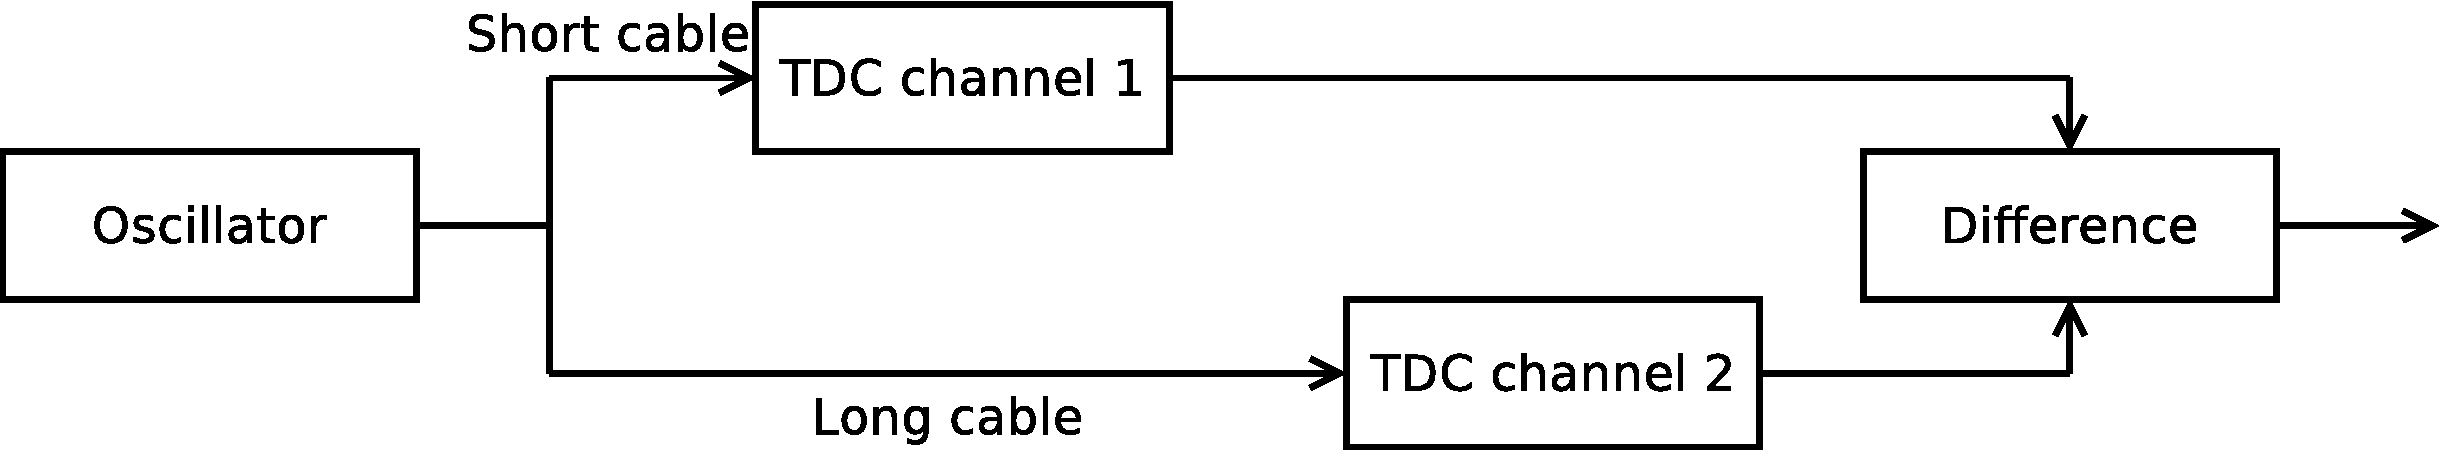
\includegraphics[width=\textwidth]{dtdc.pdf}
\caption{Principle of differential measurements.}
\label{fig:dtdc}
\end{figure}

The advantage of this technique is that it is easy to set up and does not require expensive equipment. A limitation is that the result is not affected by common-mode noise of the input path to the delay line (Figure \ref{fig:inputpath}).

We made the measurements at thermal equilibrium, with the sensor measuring 36.9375\degree C. The histogram of the results is shown in Figure \ref{fig:mhist}.

\begin{figure}[H]
\includegraphics[width=\textwidth]{mhist.pdf}
\caption{Differential measurement results.}
\label{fig:mhist}
\end{figure}

The results can be modeled with a Gaussian distribution having a mean of 2221ps (which is close to the 4ns-2ns difference in propagation times from the cables) and a standard deviation of 37ps. If we suppose that the jitter in each channel is independent and also has a Gaussian distribution, we can estimate that its standard deviation is 26ps. This means that for one channel, 95\% of the results are precise to $\pm$52ps.

\textit{Note that we obtained these results using only the TDC events from falling edges. The rising edges show a number of discrepancies that we believe to originate from signal integrity issues --- the impedances were not matched in our setup. These problems vanished when we tried routing the measurement signal path within the FPGA instead of going off-chip.}

\subsection{Temperature compensation}
Even though the influence of temperature is small (\S \ref{sec:rofreq}), we can still see the positive action of the online calibration.

After calibrating at 37\degree C, we brought the temperature to 47.875\degree C, and ran startup calibration again. We observed a significant difference between the LUT contents (figure \ref{fig:chtmlt}).

\begin{figure}[H]
\includegraphics[width=\textwidth]{chtmlt.pdf}
\caption{Difference between the LUT contents from two startup calibrations at high and low temperatures.}
\label{fig:chtmlt}
\end{figure}

The new LUT data are very close to what had been extrapolated from the 37\degree C data by the online calibration system (Figure \ref{fig:chtmht}). In fact, in this sample the difference is slightly smaller than what we had observed between two startup calibrations at the same temperature (Figure \ref{fig:scs}). This shows the good working of the online calibration system.

\begin{figure}[H]
\includegraphics[width=\textwidth]{chtmht.pdf}
\caption{Difference between the LUT contents from startup calibration and the values computed by online calibration.}
\label{fig:chtmht}
\end{figure}

\section{Final remarks}
With our system, we can expect a precision of $\pm$52ps for 95\% of the measurements. There are however several areas of improvement:
\begin{itemize}
\item Examining the startup calibration histograms reveals that almost half of the bin widths are zero. This is due to the particular propagation characteristics of carry chains, which are not the best solution for a delay line (their advantage, however, is that it is relatively easy to keep the exact same delays between runs of the place-and-route tool). It can make sense to use regular LUTs and/or general routing to implement the delay line instead, at the cost of increased design difficulty and reduced portability.
\item The carry chain is very long and this restricts its possible placements and compatibility with smaller FPGAs. Using LUTs and/or routing would also alleviate this problem.
\item There are no bins significantly larger than the others, so using ``wave union'' techniques is unlikely to lead to major improvements.
\item Multiple delay lines can work in parallel and their outputs combined, in order to average errors out.
\item The influence of the input path (Figure \ref{fig:inputpath}) was not thoroughly studied.
\end{itemize}

\end{document}
